\setlength{\parskip}{\baselineskip}
\section{Introduction}

\begin{frame}{What are Neural Networks?}
	\begin{center}
		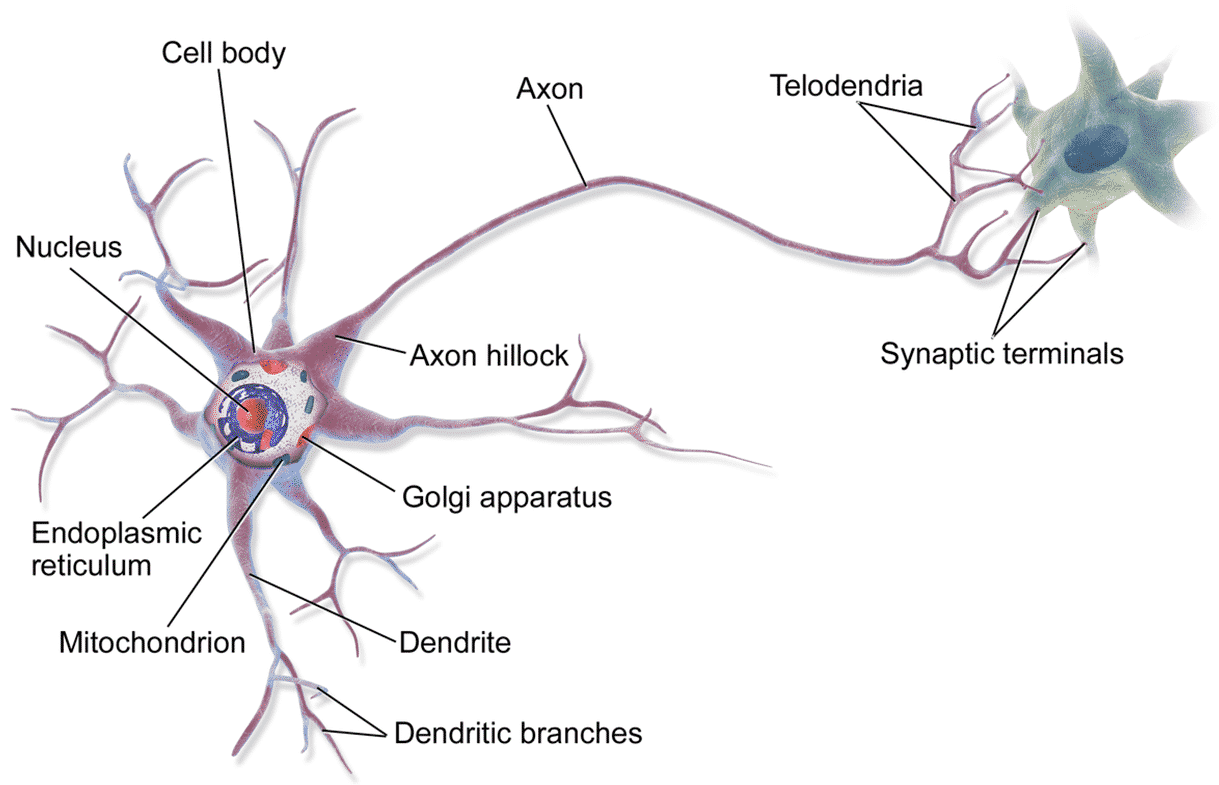
\includegraphics[width=0.6\textwidth]{../Images/CNNArchitectures/Biological-Neuron.png}\\
	\end{center}
\end{frame}

\begin{frame}{Representation of Artificial Neural Networks}
	\begin{center}
		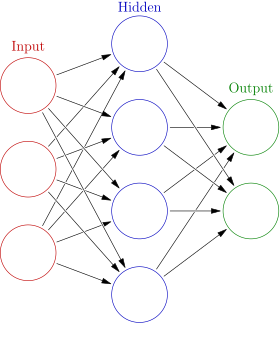
\includegraphics[width=0.3\textwidth]{../Images/CNNArchitectures/simplified-neural-network-graph.png}\\
	\end{center}
\end{frame}

\begin{frame}{ANNs on CPUs}
	\begin{minipage}{0.4\textwidth}
		\centering
		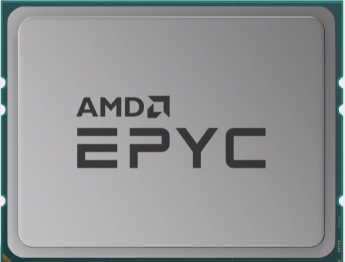
\includegraphics[width=0.6\textwidth]{../Images/Hardware/amd-epyc.png}\\
		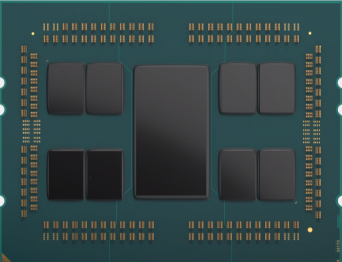
\includegraphics[width=0.6\textwidth]{../Images/Hardware/amd-epyc-dies.png}\\
		AMD Epyc 7002 series chip
	\end{minipage}%
	\begin{minipage}{0.6\textwidth}
		+ Easy development\\
		+ High clock frequency\\
		+ Advanced Vector Extensions (AVX)\\
		+ Streaming SIMD Extensions (SSE)\\\\
		- Costly\\
		- Non-scalable\\
		- Energy inefficient\\
		- Traditional Low Bandwidth Memory - up to 50 GB/s
	\end{minipage}
\end{frame}

\begin{frame}{ANNs on GPUs}
	\begin{minipage}{0.4\textwidth}
		\centering
		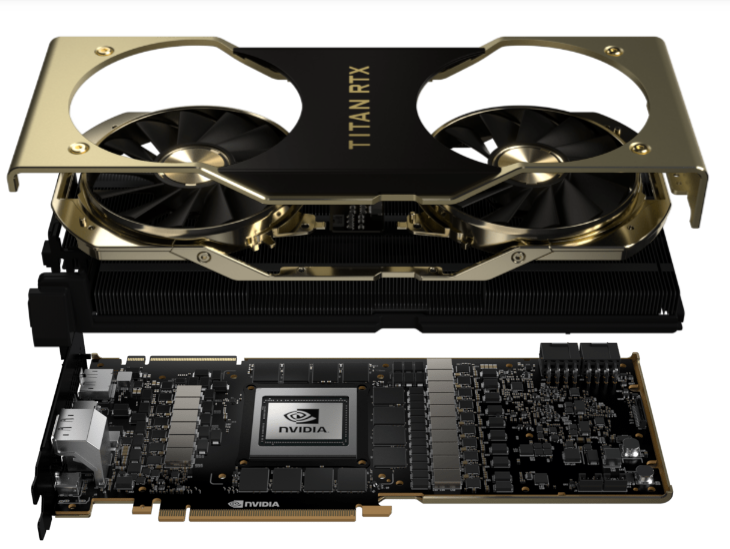
\includegraphics[width=0.9\textwidth]{../Images/Hardware/NVIDIA-Titan-RTX.png}\\
		NVIDIA Titan RTX card
	\end{minipage}%
	\begin{minipage}{0.6\textwidth}
		+ Relatively easy development\\
		+ Very high parallelism - Thousands of cores\\
		+ Specialized Tensor Cores\\
		+ Vector processing - Streaming Multiprocessors\\
		+ High Bandwidth Memory - up to 750 GB/s\\
		+ Multiple GPUs in a system\\\\
		- Very power hungry\\
		- Costly to scale up\\
		- Increased latency
	\end{minipage}
\end{frame}

\begin{frame}{ANNs on ASICs}
	\begin{minipage}{0.4\textwidth}
		\centering
		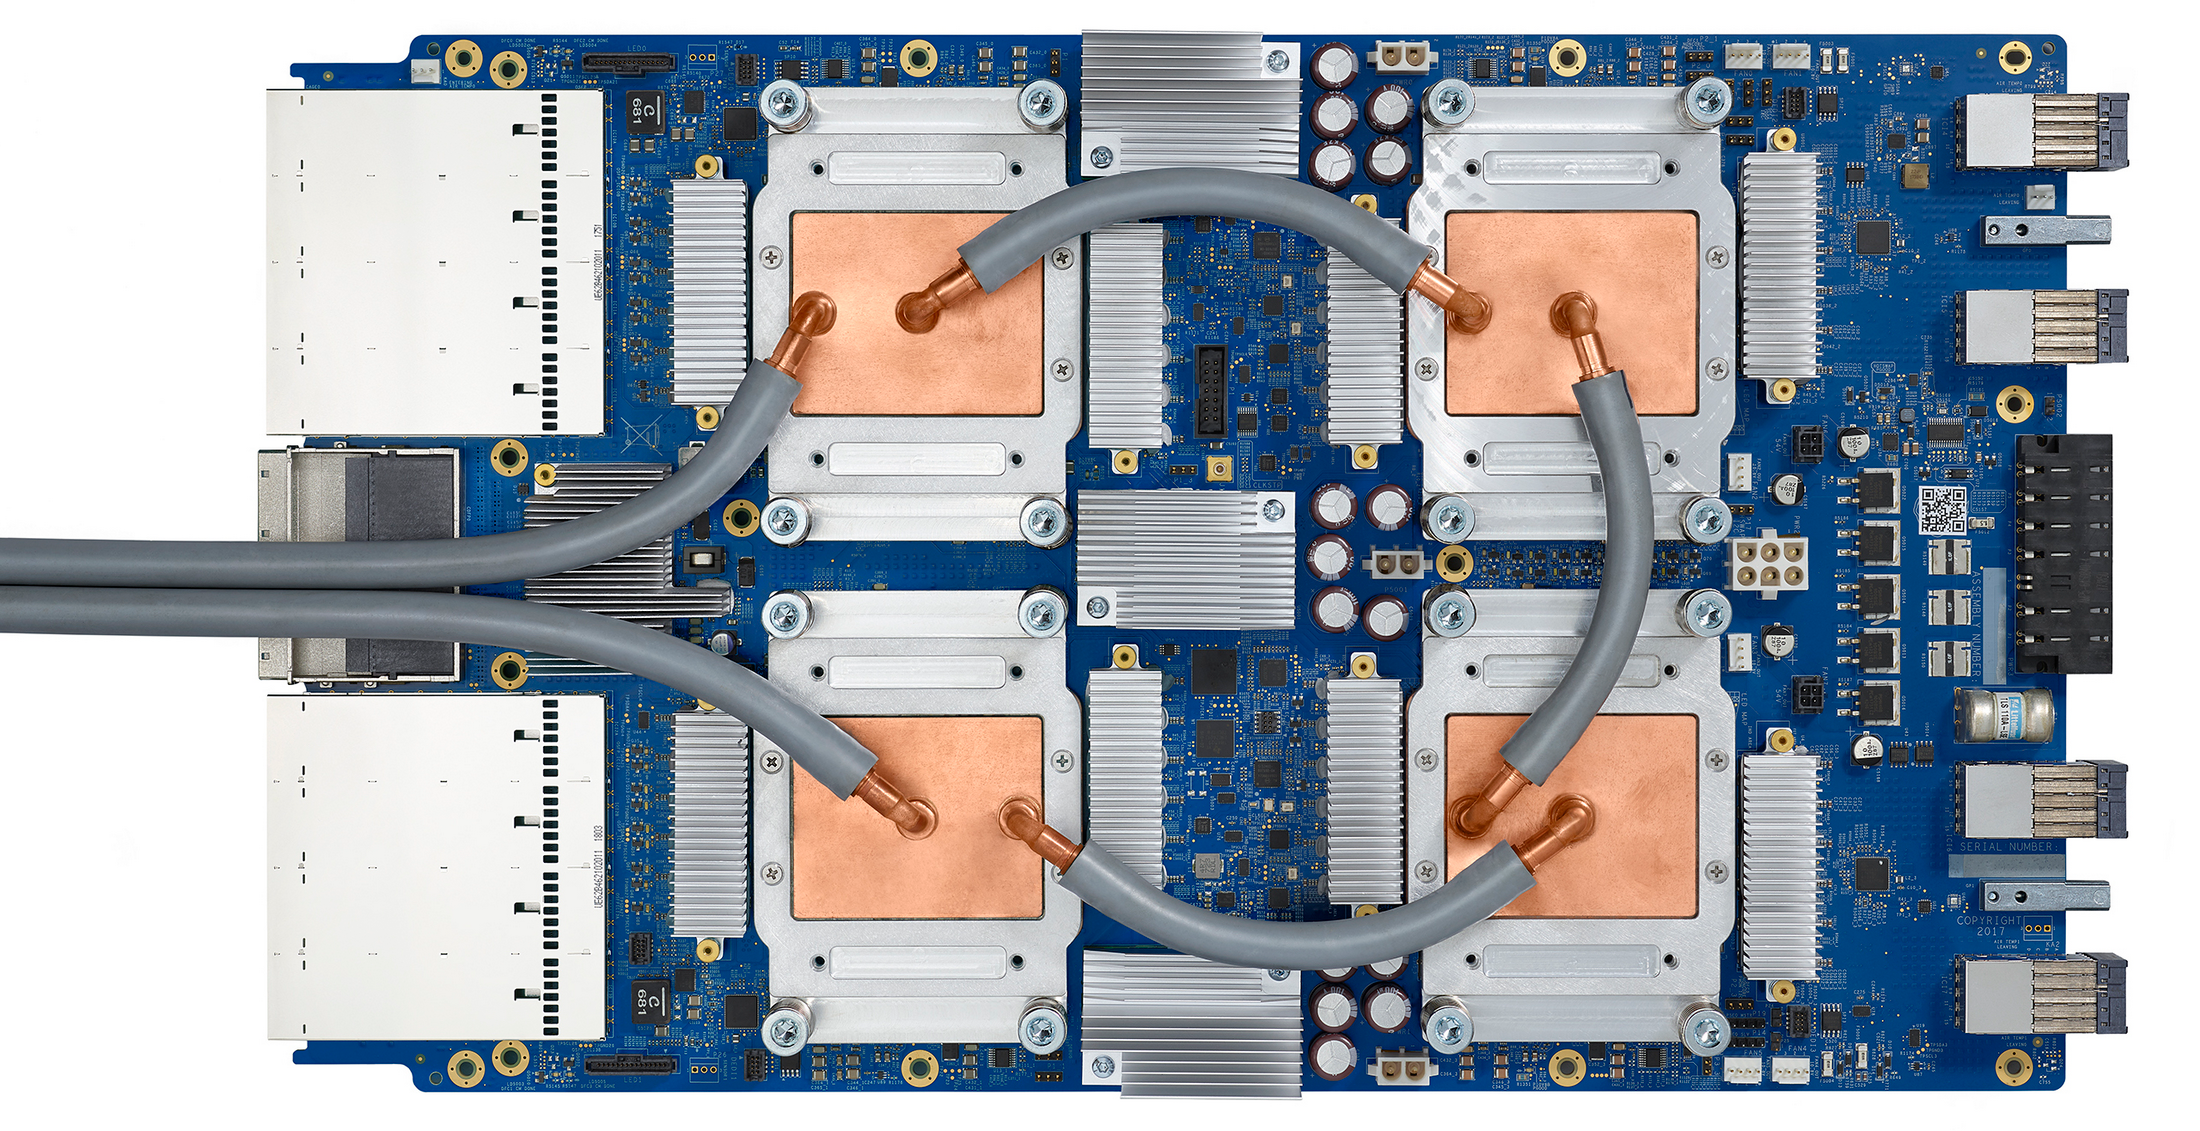
\includegraphics[width=0.9\textwidth]{../Images/Hardware/tpu-v3.png}\\
		Google TPU v3
	\end{minipage}%
	\begin{minipage}{0.6\textwidth}
		+ Best parallelism\\
		+ Lowest power \& energy consumption\\
		+ High Bandwidth Memory\\
		- Extremely expensive to design and produce\\
		- Serve a single purpose\\
		- Can become deprecated fast - AI field is still developing
	\end{minipage}
\end{frame}

\begin{frame}{ANNs on FPGAs}
	\begin{minipage}{0.4\textwidth}
		\centering
		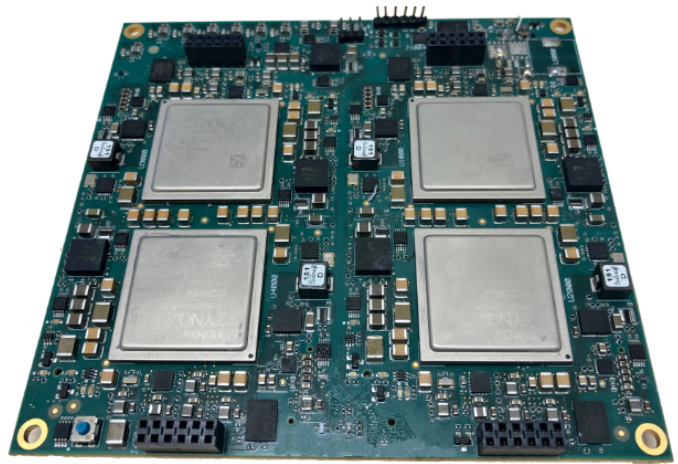
\includegraphics[width=0.6\textwidth]{../Images/Hardware/QFDB-top.png}\\
		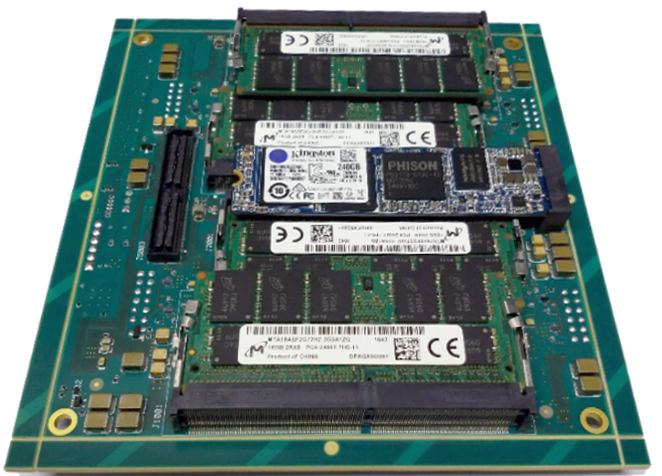
\includegraphics[width=0.6\textwidth]{../Images/Hardware/QFDB-bottom.png}\\
		FORTH QFDB
	\end{minipage}%
	\begin{minipage}{0.6\textwidth}
		+ Flexible\\
		+ Low power \& energy consumption\\
		+ Low latency\\
		+ Standalone\\\\
		- Difficult to develop\\
		- Constrained resources\\
	\end{minipage}
\end{frame}

\begin{frame}{What is Reconfigurable Logic}
	\begin{itemize}
		\item Look-Up Tables (LUTs)
		\item Flip-Flops (FFs)
		\item Block-RAM (BRAM)
		\item Ultra-RAM (URAM)
		\item Digital Signal Processing (DSP) blocks
		\item Hard Processor cores (SoC/MPSoC devices)
		\item DDR \& HBM (modern FPGAs)
	\end{itemize}
\end{frame}
